While the TreeBagger classifier performed well on this dataset, there were over 1,000 features to consider, and we were curious to see if it was possible to get similar results with only a small subset of the feature space. There are two major benefits to this:

\begin{enumerate}
\item The classifier would be trained faster. 
\item The amount of information necessary to properly classify an element would be reduced.
\end{enumerate}

If this system with a reduced feature set were implemented as a browser plug-in, this would mean faster page load times and consequently, a better user experience. 

Additionally, we felt that much of the feature data imitated what is usually done in white lists and black lists: for example, some of the features in the dataset are the source urls for images. We wanted to avoid using black lists as a reference for classification, and decided that a smaller subset of the feature space which does not consider these features was a more sincere machine learning approach to this problem.

In order to determine which features would be most useful for classification of advertisements, we first decided to look at the correlation between each of the individual features and the output\cite{feat}. The idea was that features more strongly correlated with the output are the features that are more useful for classification. The results of our feature selection choices are shown in Figure 3.

\begin{figure}[h!]
  	\label{featselall}
  	\centering
    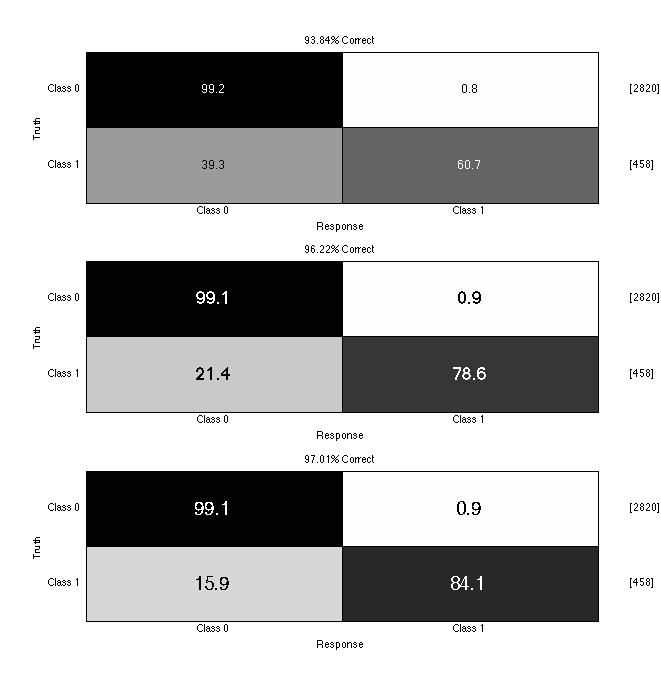
\includegraphics[width=0.5\textwidth]{Figures/featselall.jpg}
	\caption{Confusion Matrices for Selection by Entropy (Top), Selection by Correlation with Output (Middle) and Selection by PRT (Bottom)}
\end{figure}
 
We found that this subset of features achieved high correct classification with a significant reduction in the dimensionality of the feature space. It was apparent that much of the feature data was extraneous, and the problem of correct classification could be solved by only considering a some of these features.

It was also worth noting, that while the results of this classification were not perfect, it was rare that a non-advertisement was misclassified as an advertisement. This was important because we did not want to block legitimate content and instead it would be favourable if a few advertisements were allowed instead of blocking legitimate content. 

We also attempted to perform a similar feature reduction by considering the entropy of individual features. While sequential analysis of the entropy was found to be a valid method for the construction of binary decision trees, a singular calculation of the entropy, demonstrated that entropy was not an appropriate method for feature selection.

Finally, we attempted to look at more advanced feature selection techniques: using the Pattern Recognition Tool-kit's built in feature selection tool (Sequential Feature Selection), we determined the 10 best features for classification. This method works by sequentially selecting features until there is no improvement in prediction. Interestingly, more than half of these features were the same as those determined by the correlation method, though the more advanced feature selection tool had higher run times.

Interestingly, we found that for the feature selection algorithm used by the PRT we were able to achieve nearly identical results to those achieved by classification on the whole feature set. We consider this a good result as it means less overhead in a real online context. We also believe that this problem could benefit from a better feature set, but chose to work with this feature set for comparison to \cite{adeater}. We have successfully shown that we can get nearly equal classification to \cite{adeater} with a feature set less than one hundredth the dimensionality. 